%!TEX root = ../main.tex

\section{Pre-analysis} % (fold)
\label{sec:preanalysis}

For this semester we have chosen the theme \emph{Sonification}. Sonification is: 

\enquote{... the use of non-speech audio to convey information or perceptualize data.}~\cite*{Wiki2014-2}

In investigating sonification it is clear that there are more ways of sonifying data (see \enquote{Sonification Techniques} section~\ref{ssub:sonification_techniques}), depending on what kind of data is to be converted, and how that information is to be displayed and interacted with. Sonification is used in various applications and projects (see \enquote{Examples of uses of sonification} in section~\ref{ssub:examples_of_sonification}), but sonification does face some challenges in its current state. The main problem is that:

\enquote{It is difficult to provide adequate context for interpreting sonifications of data.}~\cite*{Wiki2014-2}

To see to what extend this challenge can be overcome, first one must find data to be sonified.


One area which contains different sorts of data that theoretically could be sonified is weather data. 
Some of these could be: temperature (degrees), sunny or cloudy (either or), wind speed (meters per second), visibility, precipitation (rain/sleet/snow/hail measured in millimeters). 
These data have a different range of values. 
For instance, temperature could be an array of degrees and overcast can be a boolean value of yes or no. 
This means that theoretically a lot of different sonification techniques can be applied to this kind of information. 
Aside from being sonifiable, weather information is not usually presented as sound (see Weather Data below), and could therefore possibly make for an interesting study and test of whether there could be advantages to combining non-speech audio with imagery, or possibly presenting the weather data as audio on its own, in addition to answering the question of providing sufficient context.

We would like to investigate if visually presented weather data can actually be understood, and to which degree, if converted to non-speech sound using sonification. 
Can sonification of some of these data maybe even make the weather information more understandable or relatable?
For instance, is information about wind or downpour more relatable as sound than numbers? 
These discussions have led us to the following Initial Problem Statement:

\pagebreak
\subsection{Initial Problem Statement} % (fold)
\label{sub:initial_problem_statement}

\enquote{Is it possible to successfully use sonification to convey relevant information about weather conditions as efficiently as visually represented weather conditions/data?}

% subsection initial_problem_statement (end)


\subsection{Sonification} % (fold)
\label{sub:sonification}

Now that we have an idea of what kind of data we want to sonify, we will first look into the basics of sonification. What it is, and how it is used so we can begin to plan sonification of weather data, and the best approach/technique for doing this.


\subsubsection{What is Sonification?} % (fold)
\label{ssub:what_is_sonification_}


As mentioned in the intro of this chapter (Section ~\ref{sec:preanalysis}), sonification is perceptualization of some set of data with the use of sound. 

\enquote{Sonification is a subset of the field of auditory display.}~\cite*{Walker2006}

Generally, \emph{Auditory Display} is the computer’s way of conveying information through the use of sound~\cite*{Wiki2014-3}.

An example of sonification is the traffic light junctions all around Denmark. 
When you near a crosswalk you will hear 2 different sounds. 
Both sounds are the same, but they consist of different frequencies. 
One sound (low frequency) indicates it is a red light, while the other (high frequency) indicates it is safe to walk. 
This helps blind people to know whether to cross or not, and is an example of sonification.



% subsubsection what_is_sonification_ (end)


\subsubsection{Examples of uses of sonification} % (fold)
\label{ssub:examples_of_sonification}

Now that sonification has been defined, let us delve further into the topic and see what some of the uses for sonification could be. 
A good example to start out with is the use in the medical industry.

Doctors in hospitals use stethoscopes to listen to various organs within the body of their patients. 
This can be considered a sort of sonification, as it conveys information of the patients health via sound. 
Different machines in a hospital environment also use sonification as a way of giving instant and intuitive information, while operating the equipment. 
This is for instance equipment which measures heart rate or respiration~\cite*{Sanderson2006}.
A study has shown that medical students perform better when certain information is given as sound instead of graphics on a display~\cite*[pp.23]{Barrass1999}:

\enquote{Medical students performed better in a simulated operation when eight dynamic variables about the health of the patient were presented as sounds rather than graphs, and better with sounds alone than with both sounds and graphs combined}~\cite*[pp.23]{Barrass1999}

It is not hard to imagine how distracting it must be for a doctor to constantly shift between a graph on a screen and the patient on e.g the operating table.


Sonification and auditory displays have also been implemented in aiding the blind. 
Mercator Project ~\cite*{Edwards2013}, is a project done by Keith Edwards (Research Assistant at the Georgia Tech Multimedia Computing Group), Beth Mynatt (Research Scientist at Georgia Tech Multimedia Computing Group) and Tom Rodriguez (Research Assistant at the Multimedia Computing Group), which is designed for X-Window system~\cite*{x2014} (a unix-based gui-system) and has the purpose of translating graphical interface navigation to sound cues, with the intention that blind people should be able to navigate the interface:

\enquote{The primary motivation for this work is to provide accessibility to graphical user interfaces for users who are blind or severely visually impaired.}~\cite*[p.1]{Edwards2013}

According to the report \emph{Using sonification}, by Stephen Brass (German National Research Centre for Information Technology) and Gregor Kramer (Clarity/Santa Fe Institute), some web browsers have also utilized sonification to aid blind people, by presenting e.g. download times, layout, hyperlinks and more, as sounds~\cite*[pp.24]{Barrass1999}.

An example of sonification applications in the field of science could be the ULTRA (Universal Laboratory Training and Research Aid)~\cite*{Morrison1984}.
A device created by professors David Lunney and Robert Morrison, which can audibly read out data from a range of laboratory instruments, for scientists who are visually impaired~\cite{Girvan2005}.

There have also been attempts to create location devices as a replacement for guide dogs. One such device, developed in 1965, is called the \emph{Sonic Torch}~\cite*{Ksonar}.

Basically this handheld device used sonar to capture information about the surrounding environment much like sonar on e.g. a u-boat~\cite*[1965]{Ksonar}. 
The information was then sonified to the blind person using the Sonic Torch.

\begin{figure}[!htbp]
    \centering
    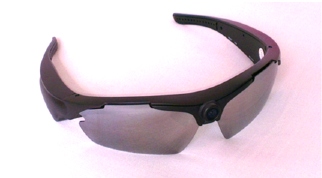
\includegraphics[width=0.7\textwidth]{images/Sonification1.png}
    \caption{vOICe by Dr. Leslie Kay.}
    \label{fig:sonification1}
\end{figure}

Another attempt at a location device, created by Dr. Peter Meijer, is called vOICe~\cite*{Meijer2014}. 
This device uses a head-mounted camera. 
The images from the camera are then sonified in a specific way, with the purpose of (over time) developing a “sixth sense” of imagery as sound by:

\enquote{...exploiting the existing multisensory processing and neural plasticity of the human brain through training and education}~\cite*{Meijer2014}


The imagery (from the camera) is translated to soundscapes and then played over headphones for the blind persons brain to interpret as spatial information~\cite*{Sandhana2003}. 
The above image shows an example of how a vOICe device can look. 
The camera in the center is what captures the image.
Generally, all these examples of technology tell us one thing. 
Technologies exist in the world where people have successfully used sonification to assist in everyday situations. 
The examples range from critical equipment dealing with life and death, to people just getting to experience what it is like to have some sort of vision. 
This tells us that sonification has a wide area of use, and focusing further on sonification techniques and how weather data is perceived and displayed will give us a good basis to work from.


There are different techniques for sonification of data. 
These will be discussed below.

% subsubsection examples_of_sonification (end)


\subsubsection{Sonification Techniques} % (fold)
\label{ssub:sonification_techniques}


The investigation of different sonification techniques will give us options and direction for when we later have to implement these techniques to sonify weather data for testing.

 % (fold)
\label{par:techniques}

Sonification techniques can be categorized into three main methods~\cite*[pp.15]{Hermann2011}:

\begin{enumerate}
    \item Event-based sonification
    \item Model-based sonification
    \item Continuous sonification
\end{enumerate}

In the book, The Sonification Handbook~\cite*{Hermann2011}, co-authors Michael Nees of Lafayette College, Easton, Pennsylvania, USA and Bruce N. Walker, Georgia Institute of Technology, Atlanta, USA, give a brief overview of the above techniques employed in sonification~\cite*[pp.16]{Hermann2011}

\subparagraph{Event-based sonification (parameter mapping):}
\label{subp:eventbased}

In event-based sonification, \linebreak changes in some values of sound (e.g. frequency, pitch etc.) happen due to to changes in given data~\cite*[pp.16]{Hermann2011}. 
Or, an event occurs in the data, which changes some parameters of the sound to make the change in the data apparent. 
Event-based sonification is usually passive, meaning it doesn’t take, or require, user input~\cite*[pp.16]{Hermann2011}.

\enquote{For instance, and alarm may be triggered by a discrete on or off threshold, or parameter mapping can be a series of discrete data which makes it seem more continuous. These event-based techniques have a passive mode of interaction.}~\cite*[pp.16]{Hermann2011}

\subparagraph{Model-based sonification:} % (fold)
\label{subp:model_based_sonification_}
In Model-based sonification a virtual model is created. 
The sonification then happens when a user interacts with the model, which then provides feedback in the form of non-speech audio.

\enquote{The user input drives the sonification. The user learns to understand the structure based on the sonic feedback of the user’s input.These types of sonification usually involves large numbers of data points and and high data dimensionality.}~\cite*[pp.17]{Hermann2011}

So where event-based sonification usually functions passively, model-based sonification requires some sort of input or user interaction.
% subparagraph model_based_sonification_ (end)

\subparagraph{continuous sonification (Audification):} % (fold)
\label{subp:audification_continues_sonification_}
Continuous sonification is “continuous” translation of incoming data. One famous example of this is the Geiger counter that conveys any level of radiation through the rate of a clicking sound~\cite*{Wiki2014-2}.

Once the Geiger counter is on, it will continuously measure and translate the incoming data from the radiation in the surrounding area into audible “clicks”.

These are the main methods of sonification, but the different techniques might not all apply to the kind of sonification required for converting weather data. 
The delimitation and choice of the sonification technique(s) most suited for our project will be discussed later (see Analysis chapter).

First we must investigate which weather data makes sense to sonify. 
This investigation will begin with looking at different weather forecast media, in order to see what different weather informations are considered to be more relevant to the general public, as it might not be relevant or necessary to cover every aspect of weather forecast information.

% subparagraph audification_continues_sonification_ (end)

% paragraph techniques (end)

% subsection sonification (end)

\subsection{Weather Data} % (fold)
\label{sub:weather_data}

Now that we have an overview of what sonification is and some methods of application, we will begin to investigate what weather information is and what types of weather information is usually decided by different sources as being more relevant to the user. 
Gathering this knowledge of popularly presented weather information will help decide, which weather information is most relevant for us to sonify in order to answer the question of how far it is possible to provide context for interpreting the sonification of, in our case, weather data.


\subsubsection{What is weather Data?} % (fold)
\label{ssub:what_is_weather_data_}
First off, what is meant by weather data? Weather data is derived from weather forecasting. 

\enquote{Weather forecasts are made by collecting quantitative data about the current state of the atmosphere on a given place and using scientific understanding of atmospheric processes to project how the atmosphere will evolve on that place.}~\cite*{Wiki2014-1}

Weather forecasts are used for different things in many different fields. Some of these include: weather warnings, traffic and road surface conditions, agriculture and of course to determine what to wear on any given day~\cite*{Wiki2014-1}.

There is a big range of different weather data, some of these are:

\begin{itemize}
     \item \textbf{Temperature/Dewpoint} - Current air temperature 2 meters above terrain.
     \item \textbf{Wind speed} - Average wind speed over 10 minutes, 10 meters above terrain.
     \item \textbf{Wind direction} - Average wind direction in degrees.
     \item \textbf{Air pressure} - Pressure at sea level measured i hPa (Hectopascal).
     \item \textbf{Humidity} - Current relative humidity measured 2 meters above terrain, measured in percent.
     \item \textbf{Precipitation} - Rain/sleet/snow/hail over the past ten minutes measured in mm.
     \item \textbf{Sun hours} - Hours with sun in a day.
     \item \textbf{Pollen Forecast} - The potency of the pollen. 
     \item \textbf{Sunrise / sunset} - Time of day where the sun rises and sets.
     \item \textbf{Cloud cover}
     \item \textbf{Wind chill} - The winds effect on air temperature.
     \item \textbf{Visibility} - How far can you see with clear line of sight.
     \item \textbf{UV-index} - Intensity of UV radiation.
     \item \textbf{Fronts} 
     \item \textbf{Source Regions} - Where the air is coming from.
     \item \textbf{Drought} - Risk of drought. Presented as a scale.
 \end{itemize}

These are just some of the weather data available in modern weather forecasting. 
Not all of these are necessarily relevant to one single individual, and weather forecasts meant for the general public (not fields of work/study that require very specific weather data) limit the amount and range of weather data presented for the sake of clarity and time (both to present the information but also the time required by the individual to get the information relevant to most). 
Below are some examples of what types of weather data have been chosen to be presented to the viewer on certain weather websites and popularly used weather applications. 
This weather information will later in the report be delimited for testing purposes of the challenge of providing adequate context for interpreting sonifications of the weather data.

% subsubsection what_is_weather_data_ (end)

\FloatBarrier
\subsubsection*{DMI.dk (Danish Meteorological Institute)} % (fold)
\label{ssub:dmi_dk_danish_meteorological_institute_}

DMI.dk is the website of the danish national meteorological institute. 
It is arguably the most well known website containing weather information, in Denmark. 
The website contains a huge amount of weather data, which makes it a bit difficult to navigate and find even the basic weather forecast of the day/week. 
Navigating through the site you will however be able to find information about the atmosphere in a given region such as: radar images of precipitation, satellite images, lightning probability, ozone measurements, snow depths, drought indexes, in addition to to the more standard weather information such as wind speed, temperature, precipitation (represented as a graph) and so on. 
However, in order to give a shorter, but more clear forecast, you have the option to get a graphically presented 7-day prognosis (Figure~\ref{fig:dmi1}

\begin{figure}[!htbp]
     \centering
     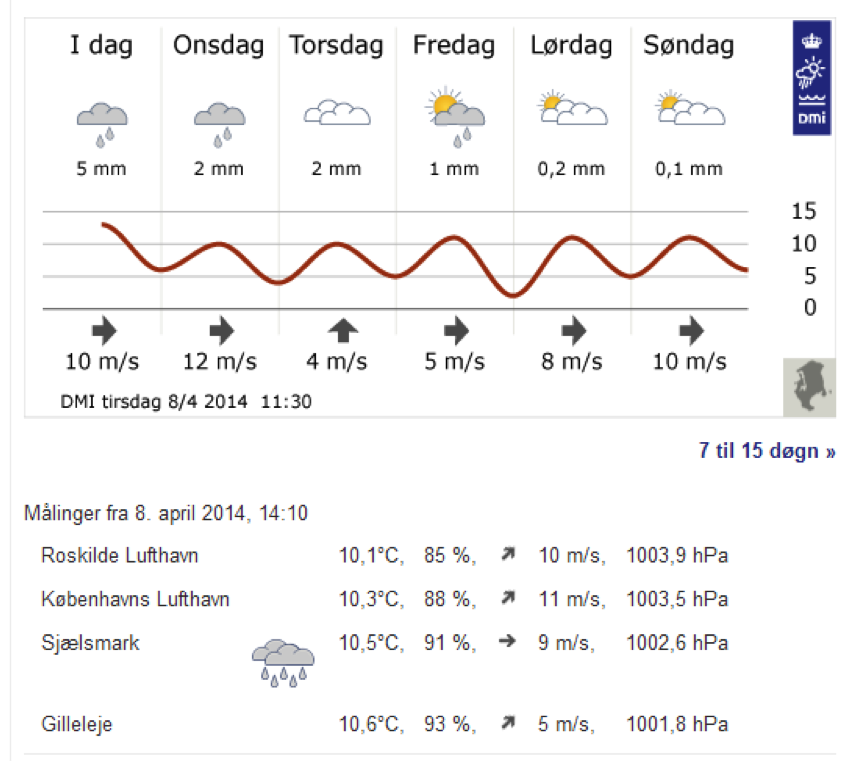
\includegraphics[width=.75\textwidth]{images/Dmi1.png}
     \caption{7-day forecast from DMI.dk}
     \label{fig:dmi1}
 \end{figure}

This is the basic weather data chosen to be relevant to the general public, and thus this is the prognosis we will be comparing with the other forecasts. 
The 7-day prognosis on DMI.dk contains information about:

\begin{itemize}
    \item Precipitation
    \item Cloud cover
    \item Temperature
    \item Wind speed
    \item Wind direction
\end{itemize}

Additionally, information measured at a certain point of the current day at predetermined locations (April 8, 2014 - 14:10) is presented:

\begin{itemize}
    \item Temperature
    \item Visibility
    \item Wind direction
    \item Wind speed
    \item Atmospheric pressure
\end{itemize}

There is also a summary of the current day’s forecast.

% subsubsection dmi_dk_danish_meteorological_institute_ (end)

\FloatBarrier
\subsubsection*{TV2 Vejret App} % (fold)
\label{ssub:tv2_vejret_app}

TV2 Vejret is a weather app developed by danish TV channel TV2 for iOS and Android. 
The app pulls weather data directly from the TV2 weather center, where the TV stations meteorologists work on predicting the weather for the TV2 news.~\footnote{https://itunes.apple.com/dk/app/tv-2-vejret/id622502267?mt=8}


The app finds the phones current location via GPS and retrieves weather information about that area. In terms of relevant data, the app gives a fairly limited amount of information (at least compared to DMI.dk), but covers the basic data such as:

\begin{itemize}
    \item Precipitation
    \item Wind speed
    \item Wind direction
    \item Sun up/down
    \item UV index
    \item Cloud cover
    \item Temperature
\end{itemize} 

From figure~\ref{fig:tv21} it is apparent that most of the information is only presented for the current time of day. 
Prognosis for the next 14 days is limited to:

\begin{itemize}
    \item Cloud cover
    \item Temperature
    \item Precipitation
    \item Wind speed
    \item Wind direction
\end{itemize}

\begin{figure}[!htbp]
    \centering
    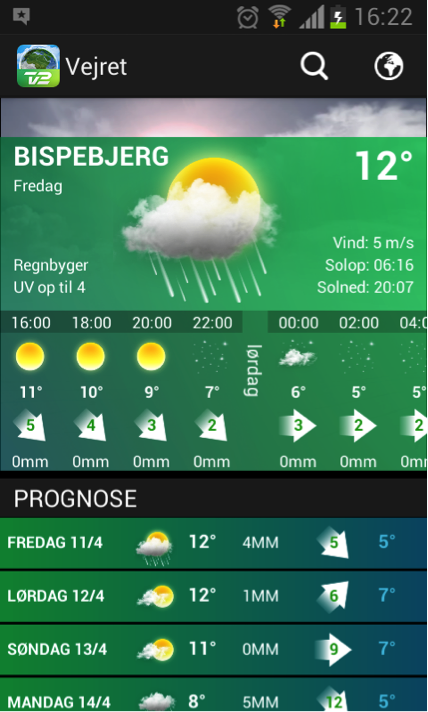
\includegraphics[width=.4\textwidth]{images/Tv21.png}
    \caption{TV2 weather app}
    \label{fig:tv21}
\end{figure}

The app does not however provide radar, heat maps or other more advanced features. 
It has the typical amount of information about the weather for an app, but where the app sets itself apart from the competition, is due to the fact that it is a TV-channel app. 
This means that the app contains video streams of the latest weather forecasts from TV, and other weather related news. 
This can be useful if you want a more detailed forecast with certain highlights about the current and forthcoming weather. 

% subsubsection tv2_vejret_app (end)

\FloatBarrier
\subsubsection*{Yahoo Weather} % (fold)
\label{ssub:yahoo_weather}

Yahoo Weather~\footnote{https://itunes.apple.com/us/app/yahoo-weather/id628677149} is an app for iOS and Android, which shows the weather in your current location, or if you want, in other locations around the world as well.
The app contains a lot of the same information that other weather applications do, it is the design of the interface and layout which sets it apart from other apps. 
The application has received the Apple Design Award~\footnote{http://en.wikipedia.org/wiki/Apple\_Design\_Awards} because of its aesthetics. 
One of the features of the design, which has gotten a lot of praise, is that the app finds images of your location on Flickr (an online image database), taking into account the time of the day and current weather condition, of your location and the photos, and uses these as the background of the weather information. 
Aside from this unique approach to visually presenting you surroundings, the interface itself is possibly the most popular feature of the app.

\pagebreak
In addition to having a very manageable interface, the app actually also contains a great deal of detailed weather information. This data includes:

\begin{itemize}
    \item Temperature
    \item Cloud cover
    \item Precipitation
    \item Probability of downpour (percentage)
    \item Wind Speed
    \item Wind direction
    \item Pressure
    \item Chill factor
    \item Humidity
    \item Visibility
    \item UV-index
    \item Sunrise/sunset
    \item Moon position
    \item Heat map
    \item Wind map
    \item Satellite map
\end{itemize}

Again, as with the TV2 Vejret app, most of the detailed information is only available for the current time on the current day. 
For the 5 and 10 day forecasts there is only information about:

\begin{itemize}
    \item Cloud cover
    \item Day/night temperature peaks
\end{itemize}

So all in all, the app does contain a lot of information about the weather, and instead of the developers delimitating the information and deciding which weather data i relevant to the user, they allow the user the option of customizing the app, deciding themselves what information is relevant. 

\begin{figure}[!htbp]
    \centering
    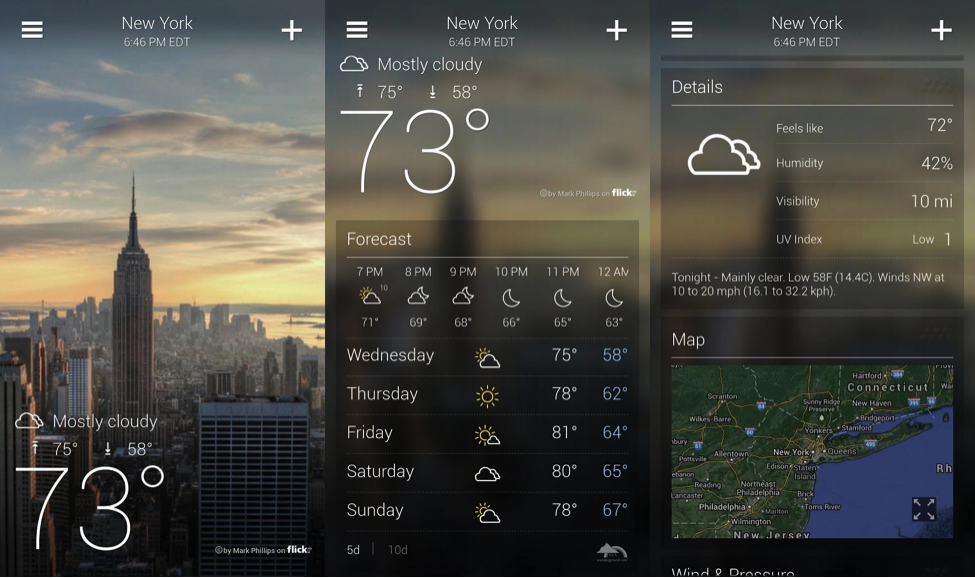
\includegraphics[width=0.95\textwidth]{images/Yahoo1.png}
    \caption{Yahoo weather app}
    \label{fig:yahoo1}
\end{figure}

% subsubsection yahoo_weather (end)

\FloatBarrier
\subsubsection*{InstaWeather} % (fold)
\label{ssub:instaweather}

InstaWeather is a weather application that focuses a lot on being a visual application. The amount of information about the weather depends on which skin to the application that you want to use. The information given can be limited to only being the temperature, a symbol that shows the weather condition and a small forecast. Some skins can also be very detailed and give information air pressure, temperature, rain, wind power and direction. The app is very customizable so you can change pictures so it feels more personal. The main feature in this application is that it borrows the picture sharing ability from Instagram. This means that the user can take a picture and send it to a friend with weather information added to the picture. 

\begin{figure}[!htbp]
    \centering
    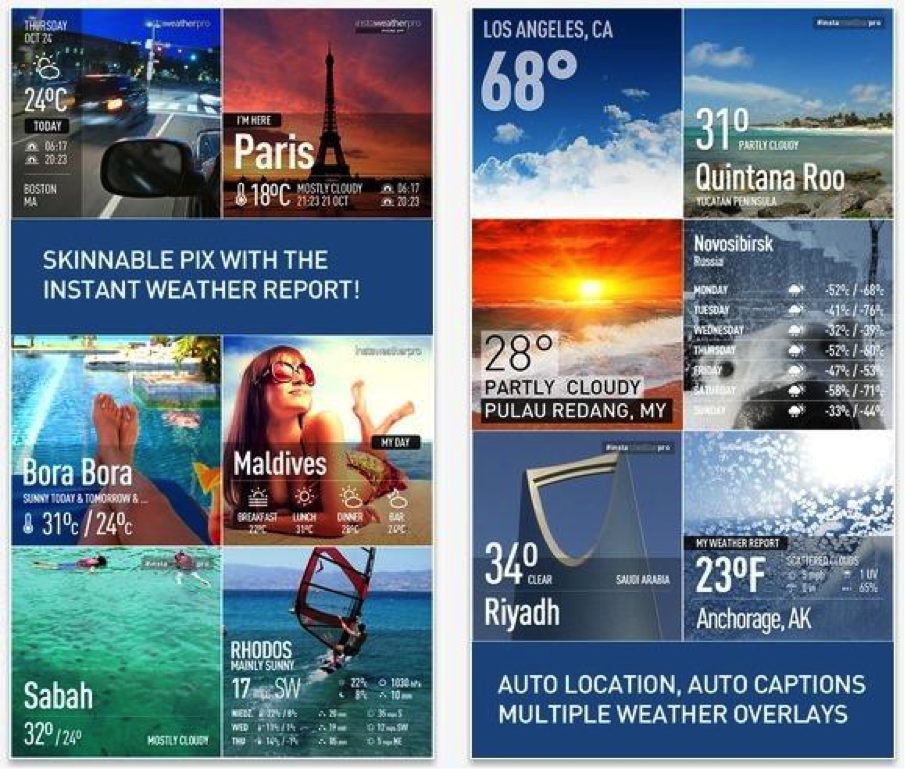
\includegraphics[width=.7\textwidth]{images/Instaweather1.png}
    \caption{InstaWeather}
    \label{fig:instaweather1}
\end{figure}

It is difficult to write about what relevant weather information is in regards to this application, because the user wholly decides for him/her self, what that is. It is in some way the most relevant weather information can be to a specific user, if that person puts in the time to customize the application for his or her needs. It does not however tell us much about what is in general considered to be chosen as relevant weather data.

Which weather information to be sonified for our test will be decided later in the Design chapter through user testing.

% subsubsection instaweather (end)

Which weather information to be sonified for our test will be decided later in the Design chapter through user testing.

% subsection weather_data (end)


\subsection{Final Problem Statement} % (fold)
\label{sub:final_problem_statement}

Now that we have an idea of the process of sonification, and having revised typical visually presented weather forecasts and their content, we have to find out whether it is possible to provide adequate context for interpretation of weather data with the use of sonification. This will be investigated by comparing to visual data presentation in order to see to what extent it is possible to provide an understanding of these data as non-speech audio. This brings us to the  final problem statement:

\enquote{To what extent is it possible to convey weather information, solely as a nonspeech auditory display, using sonification techniques, and be as intuitively understandable as visually presented weather information, where intuitive is defined as knowing by intuition?}

% subsection final_problem_statement (end)

% section preanalysis (end)
